\documentclass[9pt,a4paper]{article}
\usepackage[utf8]{inputenc}       
\usepackage[english,russian]{babel}
%\usepackage{PTSerif}                
\usepackage[pdftex]{graphicx}        
\usepackage{layout}                   
\usepackage{fancyhdr}                  
\usepackage{fullpage}                   
\usepackage{array}                       
\usepackage{longtable}                    
\usepackage{listings}
\usepackage{footnote}                       
                                             
\setlength\voffset{-1in}                      
\setlength\hoffset{-1in}                       
\setlength\topmargin{1cm}                       
\setlength\oddsidemargin{2cm}                    
\setlength\textheight{25.7cm}                     
\setlength\textwidth{17.001cm}                     
\setlength{\topskip}{1.3cm}                         
\setlength\headheight{0cm}                           
\setlength\headsep{0cm}                               
                                                       
\pagestyle{fancyplain}                                  
\fancyhf{}                                               
\cfoot{\small\em \textcopyright \hspace{0.1em} ARCСN 2013}
\rfoot{\small \thepage}

\renewcommand{\labelitemii}{$\circ$}
                                      
\title{Описание HCProbe}
\author{Александр Вершилов}

\begin{document}
\maketitle
\begin{figure}[!h]
   \centering 
   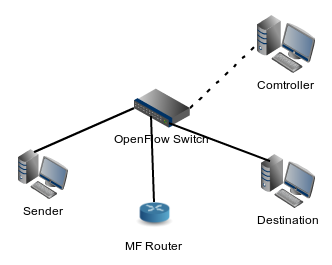
\includegraphics[width=0.3\columnwidth]{images/testcfg2.png}
\end{figure}                                                        

\tableofcontents

\pagebreak

\section{Общее описание}

\textbf{HCProbe} является реализацией библиотеки для работы с протоколом
OpenFlow на языке Haskell и предоставляет референсную реализацию софтового
openflow свича и язык для создания новых свичей, который можно использовать
для тестирования OpenFlow контроллеров.

\subsection{Перечень обозначений}

\pagebreak

\section{Подсистемы}

В библиотеке HCProbe можно выделить сделующие подсистемы:
\begin{description}
    \item[Open Flow library]  -- реализация openflow протокола
    \item[Open Flow/Ethernet] -- реализация генерации пакетов Ethernet стека
    \item[HCProbe]            -- реализация различных сетевых пакетов и референсного софтварного свича
    \item[HCProbe/EDSL]       -- доменноспецифичный язык для создания контроллеров
    \item[тесты]              -- тесты создаиня и генерации пакетов
\end{description}

\subsection{Open Flow library}

Подсистема \texttt{OpenFlow library} представляет собой поддержку протокола 
Openflow описываемого стандартом OpenFlow spec 
v1.0\footnote{http://www.openflow.org/documents/openflow-spec-v1.0.0.pdf}
для \texttt{Haskell}. Основные модули подсистемы:

\begin{description}
    \item[Network.Openflow.Types] -- реализация структур данных соотвествующая
        стуктурам данных OpenFlow протокола.
        \begin{itemize}
            \item инстансы \textbf{Binary.Read} для разбора структур;
            \item инстансы \textbf{Enum} для всех перечислений.
        \end{itemize}
    \item[Network.Openflow.Misc] -- дополнительные функции использующиеся в библиотеке
        \begin{itemize}
            \item функции подсчета CRC
            \item функции сериализации специльных типов данных
            \item функции работы с IP и MAC адресами
        \end{itemize}
    \item[Network.Openflow.Messages] -- функции серилизации и разобора сообщений OpenFlow.
\end{description}

{\emph{Реализация протокола не является полной, так реализованы не все структуры
однако расширение поддерживаемого протокола может выполняться по аналогии с
уже созданными системами}}

\subsection{OpenFlow/Ethernet}

Данная подсистема предоставляет интерфейс для создания своих типов пакетов, 
которые могут быть преобразованы в сетевые пакеты. Таким образом можно создавать
специальные тестовые пакеты с определенным заданным поведением. Основные модули:

\begin{description}
  \item[Network.Openflow.Ethernet] -- реэксопортирование всех модулей, достаточно использовать только его
  \item[Network.Openflow.ARP] -- ARP пакет
  \item[Network.Openflow.Frame] -- сетевой фрейм
  \item[Network.Openflow.IPv4]  -- IPv4 пакет
  \item[Network.Openflow.TCP]   -- TCP пакет
  \item[Network.Openflow.Types] -- внутренние типы данных
\end{description}

\subsection{HCProbe}

Исполняемый файл реализующий софтовый набор свичей, данный файл может быть использован как референсная реализация свича.

Программа \texttt{hcprobe} создает указанное количество виртуальных свичей
которые соединяются к контроллером, после чего начинаю генерировать сообщения
к контроллеру, создавая полный \texttt{TCP} пакет с подствленными маками
относящимися к портам используемым \texttt{HCProbe}. Каждый из свичей 
подсчитывает количество отправленных пакетов, количество полученных ответов,
и количество пропущенных ответов. Полученная статистика суммируется и выводится
после выполнения программы.

Потерянным считается пакет, время ожидания ответа на который превысило указанный
интервал.


\subsection{EDSL}

\subsubsection{Структура программы}
\subsubsection{Создание свича}
Свич создается командами \lstinline!switch! или \lstinline!switchOn! в первом случае
в качестве образца будет использован свич с конфигурацией по умолчанию, во-втором 
переданный свич. Таким образом командой \lstinline!switchOn! можно скопировать свич.

\begin{lstlisting}
    switch <switchIP> $ do ..
\end{lstlisting}

\subsubsection{Настройка возможностей свича}

Настройки свича проводятся в окружении \lstinline!features!, в котором можно задать
возможности свича.

\begin{lstlisting}
    switch <switchIP> $ do
      features $ do
        ..
\end{lstlisting}

Внутри настроек возможностей свича можно добавить порты командой \lstinline!addPort!.

Команда \lstinline!addMACs! добавляет список маков к свичу, при этом маки разделяются
поровну между портами.

\lstinline!clearMACs! удаляет все маки добавленные к свичу.


\subsubsection{Запуск свича}
\subsubsection{Выполнение программы}
Полсле запуска  свича он начианет выполнять переданную ему программу, данный блок 
является обычным блоком haskell кода, который может взаимодействовать со свичем
используя дополнительные команды.

\lstinline!hangOn! ожидать вечно, может быть полезно в случае если нужно тестировать
свич.

\lstinline!waitForType! ожидание определенного типа сообщения: выполнение прогаммы
будет прервано то тех пор, пока не придет сообщение указанного типа, возвращает 
полученное сообщение.

\lstinline!waitForBID! ожидание сообщения с указанным значением \texttt{buffer id}.
Возвращшает полученное сообщение.

Для генерации сообщений желательно чтобы используемые номера транзакций и буфферов 
не пересекались, для этого служат команды \lstinline!nextBID! и \lstinline!nextTID!.

\subsubsection{Отправка сообщений}

\lstinline!send!

\lstinline!sendOFPacketIn!

\lstinline!sendARPGreeting!

\subsubsection{Изменение поведения по умолчанию}

\lstinline!setUserHandler!

\section{Приложения}
\subsection{Шаблоны программирования}
\subsubsection{Ожидание нескольких сообщений}

\begin{lstlisting}
import Control.Concurrent.Async

race_ action1 action2
\end{lstlisting}

\subsection{Примеры программ}

% Идеи, что еще можно сделать с eDSL
% 1. Измениение длины пакета. Было бы здорово, если можно было бы напрямую задать значение этого поля в OF Header'е. А не влиять на нее косвенно, задавая только длину заголовка.
% 2. Генерация кривых кадров внутрь PacketIn. Также, чтобы можно было менять поля (хочу положить в Ethernet кадр IP пакет, а в заголовке написать, что это ARP), прям при создании сообщения. Сейчас для этого надо делать instance EthernetFrame.
% 3. Вообще, можно для всех типов сообщений сделать генераторы по типу putPacketIn, чтобы не приходилось этого делать через putOFData/putRaw
% 4. Очень нетривиально для человека, который не знает haskell, сделать генерацию неправильных ASCII-строк:) Но, я думаю, можно не считать это распространенным юзкейсом.
% 5. Не знаю, какую-то юзер-френдли статистику. Пока без примеров непонятно, как ее делать.
% 6. Нужен пример с несколькими свичами (с одинковой программой для каждого и с разными)

\end{document}
